% Aus dem Ordner latex kompilieren: latexmk -pdf main.tex
\documentclass[11pt,a4paper,parskip=half]{scrartcl}
\pdfminorversion=7
\usepackage[T1]{fontenc}
\usepackage[utf8]{inputenc}
\usepackage[ngerman]{babel}
\usepackage{lmodern}
\usepackage[margin=25mm]{geometry}
\usepackage{graphicx}
\usepackage{pdfpages}
\usepackage{xcolor}
\usepackage{listings}
\usepackage{booktabs,tabularx}
\usepackage[hidelinks]{hyperref}
\setlength{\emergencystretch}{2em}
\setlength{\parfillskip}{0pt plus 1fil}
\definecolor{codeBlue}{HTML}{174EA6}
\definecolor{codeGreen}{HTML}{336633}
\definecolor{codeRed}{HTML}{9C2C28}
\definecolor{codeBackground}{HTML}{F6F8FA}
\lstdefinestyle{source}{
  basicstyle=\ttfamily\footnotesize,
  keywordstyle=\color{codeBlue}\bfseries,
  commentstyle=\color{codeGreen}\itshape,
  stringstyle=\color{codeRed},
  backgroundcolor=\color{codeBackground},
  numbers=left, numberstyle=\tiny\color{gray}, numbersep=8pt,
  frame=single, rulecolor=\color{gray!35},
  xleftmargin=2em, framexleftmargin=0.5em,
  breaklines=true, breakatwhitespace=false,
  columns=fullflexible, keepspaces=true,
  showstringspaces=false, tabsize=4,
  captionpos=t,
  % pdfLaTeX: Umlaute unterstützen; Emoji-Literale als Unicode-Codepunkte zeigen.
  literate={ä}{{\"a}}1 {ö}{{\"o}}1 {ü}{{\"u}}1
           {Ä}{{\"A}}1 {Ö}{{\"O}}1 {Ü}{{\"U}}1 {ß}{{\ss}}1
           {🙂}{{[U+1F642]}}9 {🙁}{{[U+1F641]}}9
           {😉}{{[U+1F609]}}9 {😃}{{[U+1F603]}}9
}
\lstdefinestyle{cpp}{style=source,language=C++,
  morekeywords={signals,slots,emit,Q_OBJECT,QString,QObject,QWidget,
    QMainWindow,QApplication,QWebSocket,QTimer,QUrl,QVBoxLayout,QHBoxLayout,
    QLineEdit,QPushButton,QLabel,QPlainTextEdit,QMap}}
\lstdefinelanguage{CMake}{
  sensitive=true,
  morekeywords={cmake_minimum_required,project,set,find_package,if,else,endif,
    qt_add_executable,add_library,add_executable,target_link_libraries,
    set_target_properties,include,install,qt_finalize_executable},
  morecomment=[l]{\#}, morestring=[b]"
}
\lstset{style=source}
\renewcommand{\lstlistingname}{Quellcode}
\renewcommand{\lstlistlistingname}{Quellcodeverzeichnis}


% Hier persönliche Angaben ergänzen.
\newcommand{\Autor}{Simon Offenberger}
\newcommand{\Matrikelnummer}{S2410306027}
\newcommand{\Studiengang}{HSD}
\newcommand{\Abgabedatum}{\today}
\newcommand{\Quellpfad}{../RPI-ChatClient/RPI-ChatClient}
\newcommand{\todo}[1]{\textcolor{red!65!black}{\textbf{[Ergänzen: #1]}}}

% Fehlende Bilder erscheinen als beschriftete Platzhalter.
\newcommand{\bild}[3]{%
  \begin{figure}[htbp]
    \centering
    \IfFileExists{bilder/#1}{%
      \includegraphics[width=0.9\linewidth,height=0.38\textheight,keepaspectratio]{bilder/#1}%
    }{%
      \fbox{\parbox[c][42mm][c]{0.85\linewidth}{\centering
        Bild hier ergänzen\\[2mm]\texttt{\detokenize{bilder/#1}}}}%
    }
    \caption{#2}\label{#3}
  \end{figure}
}

\begin{document}
% Beide Seiten der Angabe stehen vor der Ausarbeitung.
\hypersetup{pageanchor=false}
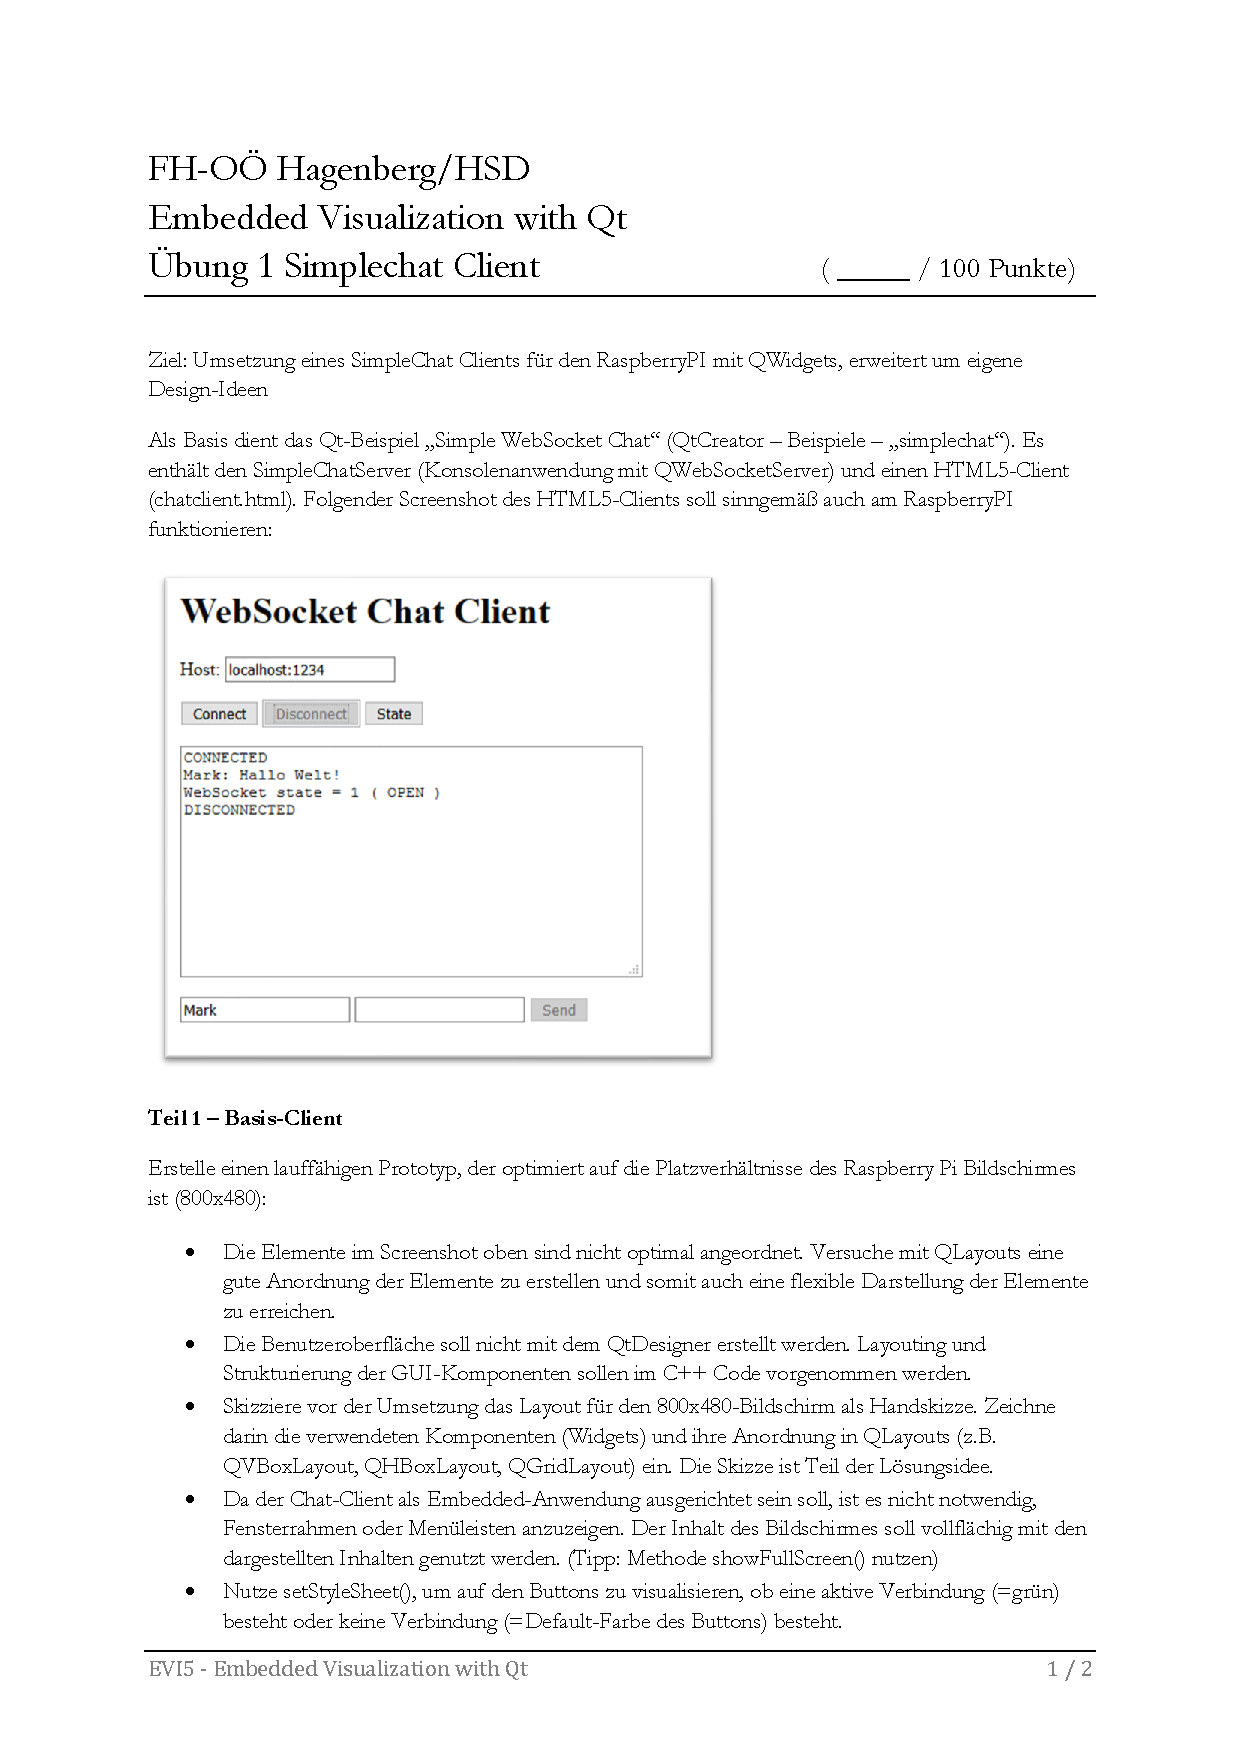
\includepdf[pages=-,pagecommand={}]{../01_EVI5_Uebung_Simplechat_2026-2.pdf}
\setcounter{page}{1}
\hypersetup{pageanchor=true}
\begin{center}
  {\LARGE\bfseries Übung 1: Simplechat Client\par}
  \medskip
  {\large Embedded Visualization with Qt\par}
  \bigskip
  \Autor\quad |\quad \Matrikelnummer\\
  \Studiengang\\
  \Abgabedatum
\end{center}
\tableofcontents
\clearpage
\section{Aufgabenstellung und Ziel}
Ziel ist ein Simplechat-Client mit Qt Widgets für einen Raspberry Pi mit
einer Bildschirmauflösung von 800\,\(\times\)\,480 Pixeln. Die Oberfläche
soll durch im C++-Code angelegte Layouts flexibel auf unterschiedliche
Fenstergrößen reagieren. Die Kommunikation erfolgt über WebSockets mit
dem Simplechat-Server. Zusätzlich werden zwei eigene Ideen umgesetzt.

\section{Lösungsidee und Aufbau}
\subsection{Layout und Handskizze}
Das zentrale Widget verwendet ein \texttt{QVBoxLayout}. Oben befinden sich
zwei horizontale Zeilen: Serveradresse mit den Schaltflächen zum Verbinden
und Trennen sowie die Eingabe des Benutzernamens. Darunter liegt der
schreibgeschützte Chatverlauf als \texttt{QPlainTextEdit}. Eine weitere
Zeile enthält das Nachrichteneingabefeld und die Senden-Schaltfläche.

\bild{handskizze.png}{Handskizze der Oberfläche mit Widgets und QLayouts.}{fig:skizze}

Für das Layout in der Skizze wurde als zentrales Layoutelement ein \texttt{QVBoxLayout} gewählt. 
In diesem vertikalen Layout befinden sich drei horizontale Layouts, die jeweils die Widgets der Zeilen enthalten.
In der ersten Zeile befinden sich die Widgets für die Serveradresse und die Buttons zum Verbinden und Trennen.
Wichtig war mir persönlich, dass hier am unteren Rand die Zeile mit der Nachrichteneingabe und der Senden-Schaltfläche ist.
Denn dieses Layout ist für die meisten Menschen vertraut, da es auch in den meisten Chatprogrammen so umgesetzt ist.

\clearpage

\subsection{Klassen und Kommunikation}
\begin{description}
  \item[\texttt{MainWindow}] Erstellt die Chat-Oberfläche im C++-Code,
    verbindet die Bedienelemente mit Slots und stellt den Verbindungszustand dar.
  \item[\texttt{Chatclient}] Kapselt den WebSocket, sendet und empfängt
    Nachrichten und steuert die automatische Wiederverbindung.
  \item[\texttt{EmojiReplacer}] Ersetzt definierte Text-Emoticons durch
    Unicode-Emojis. Die Ersetzung erfolgt beim Senden und Empfangen.
  \item[\texttt{main.cpp}] Erstellt die Anwendung, setzt die Schrift per
    Stylesheet auf 16\,pt und öffnet das Hauptfenster mit \texttt{showFullScreen()}.
\end{description}
Signale und Slots verbinden Netzwerklogik und Oberfläche. Der Client meldet
empfangene Nachrichten und Zustandsänderungen an das Hauptfenster.
Beim Senden wird der Benutzername vor die Nachricht gesetzt, die Nachricht
wird außerdem lokal an den Verlauf angehängt.

\subsection{Darstellung und Bedienung}
Bei aktiver Verbindung erscheint die Verbinden-Schaltfläche grün und zeigt
\glqq verbunden\grqq. Im getrennten Zustand wird ihr Stylesheet
zurückgesetzt. Während der Wiederverbindung ist die Anzeige gelb.
Die Nachrichteneingabe und das Senden sind nur bei aktiver Verbindung
freigeschaltet. Nachrichten können auch mit der Eingabetaste gesendet werden.

\newpage

\section{Erweiterungen aus Teil 2}
Es wurden folgende zwei Ideen aus dem Ideenkatalog umgesetzt. 

\begin{itemize}
  \item Automatische Wiederverbindung bei Verbindungsabbrüchen
  \item Emoji-Ersetzung für die Eingaben \texttt{:)}, \texttt{:(},
    \texttt{;)} und \texttt{:D}
\end{itemize}

\subsection{Idee 1: Automatische Wiederverbindung}
\textbf{Kategorie laut Ideenkatalog:} Robustheit

\textbf{Umsetzung:} Bei Verbindungsfehlern oder Verbindungsabbrüchen plant
\texttt{Chatclient} über einen einmalig auslösenden \texttt{QTimer} einen
neuen Verbindungsversuch nach 500\,ms. Die zuletzt verwendete URL bleibt
gespeichert. Weitere Fehlschläge können erneut einen Versuch auslösen.
Manuelles Trennen stoppt den Timer und deaktiviert weitere Versuche.

\textbf{Begründung:} Eine vorübergehende Netzwerkunterbrechung erfordert
dadurch keinen erneuten manuellen Verbindungsaufbau. Die gelbe Zustandsanzeige
macht den Wiederverbindungsversuch auf dem Embedded-Gerät sichtbar.

\bild{idee-reconnect.png}{Desktop: Wiederverbindungsversuch nach dem Stoppen des lokalen Servers.}{fig:reconnect}
\newpage
\subsection{Idee 2: Emoji-Ersetzung}
\textbf{Kategorie laut Ideenkatalog:} Darstellung

\textbf{Umsetzung:} \texttt{EmojiReplacer} ersetzt die Eingaben
\texttt{:)}, \texttt{:(}, \texttt{;)} und \texttt{:D} anhand einer
\texttt{QMap}. Die Ersetzung erfolgt sowohl vor dem Senden als auch beim
Anzeigen empfangener Nachrichten.

\textbf{Begründung:} Häufig verwendete Emojis lassen sich über kurze
Tastatureingaben erzeugen. Eine zusätzliche Auswahloberfläche beansprucht
dadurch keinen Platz auf dem kleinen Bildschirm.

\bild{idee-emojis.png}{Desktop: Alle vier Emoticons werden beim Senden und Empfangen ersetzt. Die Eingabezeile zeigt die ursprünglichen Kurzformen.}{fig:emojis}
\newpage
\section{Ausführung und Nachweise}

\subsection{Ausführung auf dem Raspberry Pi}

Nun wurde der Chat-Client auf dem Raspberry Pi ausgeführt.
Hier ist zu erkennen, dass die Oberfläche auf dem kleinen Bildschirm gut lesbar ist und die Bedienung mit den Fingern gut funktioniert.
Hierbei ist es wichtig, dass die Buttons und Eingabefelder groß genug sind, um sie mit den Fingern gut bedienen zu können.
Außerdem soll das Textfeld für den Chatverlauf groß genug sein, um die Nachrichten gut lesen zu können.

\bild{normaleVerbindung_PI.jpeg}{Ausgeführter Chat-Client auf dem Raspberry Pi.}{fig:rpi}

\bild{reconnect.jpeg}{Reconnect - Wiederverbindungsversuch am Raspberry Pi.}{fig:rpi}

Für die Emoji-Ersetzung auf dem Raspberry Pi musste eine Schriftart mit Emoji-Unterstützung installiert werden.
Die Schriftart \texttt{Noto Color Emoji} wurde über scp auf den Raspberry Pi kopiert und anschließend eingebunden.

Hier wurde die Schriftart mit folgenden Befehlen installiert:
\begin{lstlisting}[language=bash]
mkdir -p /usr/share/fonts/truetype/noto

cp /tmp/NotoColorEmoji.ttf \
   /usr/share/fonts/truetype/noto/

chmod 644 /usr/share/fonts/truetype/noto/NotoColorEmoji.ttf
\end{lstlisting}

\bild{Emojies.jpeg}{Emoji-Ersetzung auf dem Raspberry Pi.}{fig:rpi}


\subsection{Flexible Fenstergrößen am Desktop}
Für die Desktop-Aufnahmen wurde das laufende Fenster mittels mit \texttt{show()} in den Fenstermodus versetzt und
auf 800 x 480 beziehungsweise ca. 1200 x 720 Pixel skaliert.
Bei größerem Fenster wachsen insbesondere der Chatverlauf und die
Eingabefelder, die Anordnung der Bedienelemente bleibt erhalten.
Ein zweiter WebSocket-Testclient bestätigte den Nachrichtenaustausch.
\bild{desktop-klein.png}{Desktop-Ausführung mit 800 x 480 Pixeln Fensterinhalt.}{fig:desktop-klein}
\bild{desktop-gross.png}{Desktop-Ausführung mit 1200 x 720 Pixeln Fensterinhalt.}{fig:desktop-gross}



\clearpage
\appendix
\section{Vollständiger Projektquellcode}
\lstlistoflistings

\subsection{Projektkonfiguration}
\lstinputlisting[language=CMake,caption={CMakeLists.txt}]{\Quellpfad/CMakeLists.txt}
\lstinputlisting[language={},caption={CMakePresets.json}]{\Quellpfad/CMakePresets.json}

\clearpage
\subsection{Programmeinstieg}
\lstinputlisting[style=cpp,caption={main.cpp}]{\Quellpfad/main.cpp}

\subsection{WebSocket-Client}
\lstinputlisting[style=cpp,caption={chatclient.h}]{\Quellpfad/chatclient.h}
\lstinputlisting[style=cpp,caption={chatclient.cpp}]{\Quellpfad/chatclient.cpp}

\clearpage
\subsection{Benutzeroberfläche}
\lstinputlisting[style=cpp,caption={mainwindow.h}]{\Quellpfad/mainwindow.h}
\lstinputlisting[style=cpp,caption={mainwindow.cpp}]{\Quellpfad/mainwindow.cpp}
\lstinputlisting[language=XML,caption={mainwindow.ui}]{\Quellpfad/mainwindow.ui}

\clearpage
\subsection{Emoji-Ersetzung}
\lstinputlisting[style=cpp,caption={emojireplacer.h}]{\Quellpfad/emojireplacer.h}
\lstinputlisting[style=cpp,caption={emojireplacer.cpp}]{\Quellpfad/emojireplacer.cpp}

\end{document}
